\documentclass[../main.tex]{subfiles}

% \date{September 6 to September 8 and September 11 to September 15}
% \title{Introduction to limits}
% Stewart (9E). Sections 2.2, 2.3 and 2.4. Pages 83 to 114.

\begin{document}

\textbf{Notes}. These GeoGebra activities gradually introduce limits with associated techniques.
\begin{itemize}
  \item These GeoGebra activities \emph{do not} work well on tablets and phones.%You should bring a laptop to class.
  \item The GeoGebra worksheet is available at \url{https://www.geogebra.org/calculator/xzawxtcy}.
  \item It is recommended to perform these activities in small groups.
\end{itemize}


\textbf{Objectives}.
At the end of the lecture, you should be able to
\begin{itemize}
  \item distinguish evaluating a limit from evaluating a function,
  \item estimate one-sided and two-sided limits using graphs and data tables,
  \item recognize vertical asymptotes of a function,
  \item evaluate two-sided limits for functions, %continuous functions, 
  \item distinguish limit does not exist from limit going to an infinity,
  \item use limit laws to evaluate limits,
  \item evaluate the limit of a rational function approaching an undefined number,
  \item use squeeze theorem to evaluate limits, and
  \item use the delta-epsilon definition of limits. %to verify a limit.
\end{itemize}

\textbf{instruction} (How to estimate an \emph{one-sided} limit using the GeoGebra worksheet)
\begin{enumerate}[label=(\alph*)]
  \item From the limit notation, identify \(f(t)\), the limiting number \(a\), and the direction. Choose the correct options from the drop-down menus. Then click the \raisebox{-0.5em}{\includegraphics[height=1.6em]{week1-reset}} button. You might need to right-click (on any blank space) and click \raisebox{-0.5em}{{\includegraphics[height=1.5em]{week1-zoom-to-fit}}} once.
  \item Move the blue diamond \raisebox{-0.5em}{\includegraphics[height=1.5em]{week1-blue-diamond}} on the horizontal axis closer to the limiting number \(a\). As \(t\) moves closer to \(a\), does \(f(t)\) appear to get closer to a certain number? If this number exists, then it is the desired limit! %Zoom in or zoom out if necessary. 
  \item[\faIcon{comments}] Which direction does \(t\) \emph{approach} the limiting number \(a\)? From left to right? Or from right to left?
  \item[\faIcon{comments}] Do you need the value \(f(t)\) at \(t = a\) to find this limit?
\end{enumerate}
\clearpage

\begin{outline}{2.2}{Notation and one-sided limits}{page}
  \label{act:one-sided}
  \begin{enumerate}
    \item Review polynomials and root functions, their domains, and their graphs.
    \item Review piecewise functions and their notation.  Discuss their domains and graphs.
    \item \textbf{The intuitive definition of one-sided limits}. Suppose \(f(x)\) is defined when \(x\) is near the number \(a\).
          \begin{itemize}
            \item We write \(\lim_{x \to a^{-}} f(x) = L\) and say that the \emph{left-hand limit of} \(f(x)\) as \(x\) approaches \(a\) is equal to \(L\) if we can make the values of \(f(x)\) arbitrarily close to \(L\) by restricting \(x\) to be sufficiently close to \(a\) with \(x < a\).
            \item We write \(\lim_{x \to a^{+}} f(x) = L\) and say that the \emph{right-hand limit of} \(f(x)\) as \(x\) approaches \(a\) is equal to \(L\) if we can make the values of \(f(x)\) arbitrarily close to \(L\) by restricting \(x\) to be sufficiently close to \(a\) with \(x > a\).
          \end{itemize}
    \item The letter \(x\) below the limit symbol \(\lim_{x \to a^{+}} f(x)\) is called a \emph{dummy variable}. It means we can change it to whatever we want as long as we change all occurances of \(x\) to the new symbol. After such change, the meaning of the limit symbol does not change. For example, we can change \(x\) to \(t\) and we would have an equality
          \[
            \lim_{x \to a^{-}} f(x) = \lim_{t \to a^{-}} f(t).
          \]
          However, we must not change \(a\) since it is a fixed value.
    \item Use Table~\ref{table:limits_introduction} to estimate the limit of \(t^{2}\) as \(t\) approaches \(1\) from the left and from the right.
          \begin{table}[h]
            \centering
            % \includegraphics{../standalones/table_t_squared}
            \begin{tabular}{l | l}
              \(t\)      & \(t^{2}\)  \\
              \midrule
              \(0.9\)    & \(0.81\)   \\
              \(0.95\)   & \(0.9025\) \\
              \(0.99\)   & \(0.9801\) \\
              \(0.999\)  & \(0.998\)  \\
              \(0.9999\) & \(0.9998\) \\
              \(1.0001\) & \(1.0002\) \\
              \(1.001\)  & \(1.002\)  \\
              \(1.01\)   & \(1.0201\) \\
              \(1.05\)   & \(1.1025\) \\
              \(1.1\)    & \(1.21\)   \\
            \end{tabular}
            \label{table:limits_introduction}
            \caption{The function \(t^{2}\) as a table.}
          \end{table}
    \item Use the GeoGebra worksheet to estimate \(\lim_{t \to 1^{-}} t^{2}\) and \(\lim_{t \to 1^{+}} t^{2}\).
    \item \label{part:piecewise} Choose the first function in the drop-down menu for \(f(t)\). This is a piecewise function defined by
          \[
            f(t) =
            \begin{cases}
              1, & \text{if } t < 2, \\
              2, & \text{otherwise}.
            \end{cases}
          \]
          Use the GeoGebra worksheet to estimate its \emph{left and right} limits at \(2\). %Do the left and right limits agree?
    \item There are three parts in the limit notation. Left and right limits do not always agree. The function value at the limiting number \(a\) is \emph{not} needed to \emph{evaluate} a limit.
  \end{enumerate}
\end{outline}

\begin{outline}{sec}{Two-sided limits and limits of continuous functions}{page}
  \label{act:two-sided}
  \begin{enumerate}
    \item Review \(\sin(t)\) and \(\cos(t)\), their domains, and their graphs.
    \item The intuitive definition of a (two-sided) limit. Suppose \(f(x)\) is defined when \(x\) is near the number \(a\). Then we write \(\lim_{x \to a} f(x) = L\) and say ``the limit of \(f(x)\), as \(x\) approaches \(a\), equals \(L\)'' if we can make the values of \(f(x)\) arbitrarily close to \(L\) by restricting \(x\) to be sufficiently close to \(a\) but not equal to \(a\).
    \item One-sided limits and two-sided limits are related as follows.
          \begin{mdframed}[style=simple]
            \[
              \lim_{x \to a} f(x) = L
              \quad\text{if and only if}\quad
              \lim_{x \to a^{-}} f(x) = L \text{ and }
              \lim_{x \to a^{+}} f(x) = L.
            \]
          \end{mdframed}
    \item Use the GeoGebra worksheet to estimate \(\lim_{t \to \pi/2} \sin(t)\). Remember to find both left and right limits.
    \item Identify the limiting number \(a\) from the notation. Does the limit agree with \(\sin(a)\)?
    \item What other functions are \emph{continuous} like \(\sin(t)\)? Try to remember the graphs of the functions you have learned so far. You can also play with the functions in the GeoGebra worksheet.
    \item For the piecewise function in Outline~\ref{act:one-sided} part \eqref{part:piecewise}, does the limit exist at \(a = 2\)?
    \item For everywhere continuous elementary functions such as polynomials, \(e^{t}\), \(\sin(t)\), and \(\cos(t)\), we can use direct substitution to evaluate their limits \emph{anywhere}. Its left and right limits must agree for a two-sided limit to exist.
  \end{enumerate}

  Note: Intuitively, a function is continuous if one can draw its graph without lifting the pen. We will learn a precise definition of continuity in Section 2.5.
\end{outline}


\begin{outline}{sec}{Infinite limits and vertical asymptotes}{page}
  \label{act:infinity}
  \begin{enumerate}
    \item Review \(\tan(t)\), its domain and its graph.
    \item Use the GeoGebra worksheet to estimate \(\lim_{t \to (\pi/2)^{-}} \tan(t)\). Zoom out if necessary. Does \(\tan(t)\) get closer to any particular number?
    \item Use the GeoGebra worksheet to estimate \(\lim_{t \to (\pi/4)^{+}} \tan(t)\). Zoom out if necessary. Does \(\tan(t)\) get closer to any particular number?
    \item A vertical line \(t = a\) is a \emph{vertical asymptote} of a function \(f(t)\) if one of its one-sided limit as \(t\) approaches \(a\) goes to an infinity.
    \item Identify the vertical asymptotes of \(\tan(t)\).
    \item If the limit of \(g(t)\) as \(t\) approaches \(a\) goes to an infinity, then its corresponding limit goes to \(+ \infty\) or \(- \infty\). If \(a\) is neither a left nor a right vertical asymptote of \(g(t)\), then \emph{more work} is required to evaluate its corresponding limit as \(t\) approaches \(a\).
    \item At the moment, ``the limit does not exist'' means one of two things, or both.  (1) A one-sided limit goes to an infinity. (2) The left and right limits disagree. (3) There are other ways that a limit does not exist.
  \end{enumerate}
\end{outline}


\begin{outline}{sec}{Limit laws}{page}
  \label{outline:limit-laws}
  \begin{enumerate}
    % \item \textbf{Theorem.} The limit of a sum, a difference, a product, a power and a quotient (if well-defined) of functions is the sum, the difference, the product, the power and the quotient (if well-defined) of their limits respectively.  This \emph{requires} both limits exist.
    % \item \textbf{Theorem.} If \(\lim_{t \to a} f(t)\) exists, then \(\sqrt[n]{\lim_{t \to a} f(t)} = \lim_{t \to a} \sqrt[n]{f(t)}\) for any positive integer \(n\). If \(n\) is even, then we also require \(\lim_{t \to a} f(t) \ge 0\)
    \item Discuss limit laws for addition, subtraction, multiplication by a constant, multiplication,  quotient, powers, roots.

    \item If a function \(f\) is a polynomial, a rational function, a root function, \(e^{t}\), \(\sin(t)\), or \(\cos(t)\) \emph{and} a number \(a\) is in the domain of \(f\), then we can use direct substitution to evaluate the limit of a function \(f(t)\) as \(t\) approaches \(a\). Direct substitution works for these functions on their domains.
          %  \item {Limits interact with familiar algebraic operations nicely.}
          % \item {Direct substitution works for elementary functions on their domains.}
  \end{enumerate}
\end{outline}

\begin{outline}{sec}{Evaluating limits of quotients and rational functions}{page}

  \begin{enumerate}
    \item Review quotients and their domains. Highlight that rational functions are special cases of quotients.
    \item Consider the function \[\frac{t^{2} - 3t + 2}{t-2}.\] Without factoring or simplifying, is it possible to evaluate it at \(2\)? Is \(\frac{t^{2} - 3t + 2}{t-2}\) defined at \(t = 2\)?
    \item Use the GeoGebra worksheet to estimate \({\lim_{t \to 2}} \frac{t^{2} - 3t + 2}{t-2}\). Remember to find both left and right limits.
          % \item Factor the numerator of \(\frac{t^{2} - 3t + 2}{t-2}\) so that you can cancel \(t-2\) to obtain a new function \(t-1\). Evaluate \(\lim_{t \to 2} t-1\). Does \(\lim_{t \to 2} t-1\) agree with \({\lim_{t \to 2}} \frac{t^{2} - 3t + 2}{t-2}\)? 
          % \item Use the GeoGebra worksheet to estimate \({\lim_{t \to 3}} \frac{t^{2} - 3t + 2}{t-2}\). Remember you have to evaluate both left and right limits. \reflection{Is the discontinuity at \(t = 2\) relevant when the limiting value is \(a = 3\)?}
    \item Evaluate \({\lim_{t \to 2}} \frac{t^{2} - 3t + 2}{t-2}\) by factoring the numerator then looking for a cancellation.
    \item Evaluate \({\lim_{t \to 3}} \frac{t^{2} - 3t + 2}{t-2}\). Is the discontinuity at \(t = 2\) relevant when the limiting value is \(a = 3\)?
    \item Evaluate \({\lim_{t \to 0}} \frac{\sqrt{t^{2} + 1} - 1}{t^{2}}\) by rationalizing the numerator then looking for a cancellation.
    \item To evaluate the limit of a rational function or a quotient \(f(t)\) as \(t\) approaches \(a\) and \(a\) is in the domain of \(f\), use direct substitution.
    \item To evaluate the limit of a quotient \(\frac{p(t)}{q(t)}\) as \(t\) approaches \(a\) and \(a\) is \emph{not} in the domain of \(\frac{p(t)}{q(t)}\), direct substitution \emph{no longer works}. Try factoring or rationalizing to find cancellation. Notice cancellation must be performed \emph{within} the limit notation.
  \end{enumerate}
  Note: Later in the semester, we will learn a related method called \textit{L'H{\^o}pital's Rule} in Section 4.4.
\end{outline}


\begin{outline}{sec}{The Squeeze Theorem}{page}
  \begin{enumerate}
    \item Review inequalities involving trigonometric functions.
    \item The Squeeze Theorem states the following.
          \begin{mdframed}[style=simple]
            Let \(f(x) \le g(x) \le h(x)\) when \(x\) is near \(a\) (except possibly at \(a\)) and
            \[
              \lim_{x \to a}f(x) = \lim_{x \to a} h(x) = L,
            \]
            then \({\lim_{x \to a}} g(x) = L\).
          \end{mdframed}
    \item Use the Squeeze Theorem to show \({\lim_{x \to 0}} x \sin\left( \frac{1}{x} \right) = 0\). Highlight the application of the Squeeze Theorem on the graph of \(x \sin(\frac{1}{x})\) near \(0\). See Figure~\ref{fig:squeeze}.
          \begin{figure}[h!]
            \centering
            % \includegraphics[height=1.2in]{plot_squeeze}
            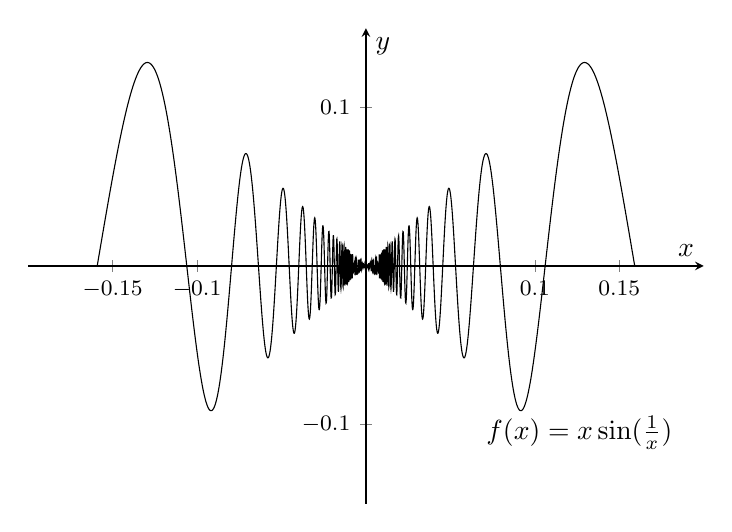
\begin{tikzpicture}
              \begin{axis}[
                  thin,
                  xtick={-0.15, -0.1, 0.1, 0.15},
                  axis lines=middle,
                  xlabel=\(x\),
                  ylabel=\(y\),
                  tick label style={font=\footnotesize},
                  width=4in, height=3in,
                  xmin=-0.2, xmax=0.2,
                  ymin=-0.15, ymax=0.15
                ]
                \addplot[blue, domain={-1/(2*pi)}:{1/(2*pi)}, samples=2000, smooth, black]{x * sin(deg(1/x))};
              \end{axis}
              \node at (7, 0.9) {\(f(x) = x \sin(\frac{1}{x})\)};
            \end{tikzpicture}
            \caption{The graph of \(x \sin(\frac{1}{x})\) near \(0\).}
            \label{fig:squeeze}
          \end{figure}

    \item Suggested problem:
          \begin{enumerate}
            \item Suppose \(x + 1 \le h(x) \le x^{3} - 2 x + 3\). Find \({\lim_{x \to 1}} h(x)\).
          \end{enumerate}
    \item The Squeeze Theorem can be used to evaluate limit of \(\lim_{x \to a} h(x)\) when \(h(x)\) is ``sandwiched'' between two functions \(f(x) \le h(x) \le g(x)\) \emph{as long as} the limits of \(f(x)\) and \(g(x)\) as \(x\) approaches \(a\) agree.
  \end{enumerate}
\end{outline}

\begin{outline}{sec}{Review absolute values and intervals}{page}
  Let \(t\) be a variable, \(c\) be a fixed number, and \(r\) be a fixed \emph{positive} number. The inequality \(|t - c| < r\) has a geometric interpretation. When sketching an interval, draw a small circle \(\circ\) to exclude endpoints if necessary.
  \begin{enumerate}
    \item On the number line below, highlight the interval indicated by \(|t| < 2\).
          \begin{center}
            % \includegraphics{../standalones/build/plot_review_abs}
            \begin{tikzpicture}
              \draw[->] (-6,0) -- (6,0) node[right] {\small \(t\)};
              \foreach \n in {-5,...,5} {
                  \draw (\n, 0.1) -- (\n, -0.1) node[below] {\small \(\n\)};
                }
            \end{tikzpicture}
          \end{center}

    \item On the number line below, highlight the interval indicated by \(|t - 1| < 2\).
          \begin{center}
            \begin{tikzpicture}
              \draw[->] (-6,0) -- (6,0) node[right] {\small \(t\)};
              \foreach \n in {-5,...,5} {
                  \draw (\n, 0.1) -- (\n, -0.1) node[below] {\small \(\n\)};
                }
            \end{tikzpicture}
          \end{center}

    \item On the number line below, highlight the interval indicated by \(|t + 1| < 2\).
          \begin{center}
            \begin{tikzpicture}
              \draw[->] (-6,0) -- (6,0) node[right] {\small \(t\)};
              \foreach \n in {-5,...,5} {
                  \draw (\n, 0.1) -- (\n, -0.1) node[below] {\small \(\n\)};
                }
            \end{tikzpicture}
          \end{center}
    \item The inequality \(|t - c| < r\) is the open interval \((c - r, c + r)\). It is centred at \(c\) and includes all numbers (strictly) less than \(r\) away from \(c\). Its length is \(2r\).
  \end{enumerate}
\end{outline}

\begin{outline}{sec}{The delta-epsilon definition of limits}{page}

  \begin{enumerate}
    \item Review absolute values and inequalities  of the form \(|t - c| < r\) (where \(t\) is a variable, \(c\) is a fixed number, and \(r\) is a fixed \emph{positive} number).
    \item \textbf{Definition} (The delta-epsilon definition of limit).
          \begin{mdframed}[style=simple]
            Let \(f(t)\) be a function and \(a\) be a real number. A candidate limit \(L\), also a real number, is the limit of \(f(t)\) as \(t\) approaches \(a\) if
            \begin{center}
              for every \(\varepsilon > 0\), there exists a \(\delta > 0\) \textit{such that} \(|t - a| < \delta\) implies \(|f(t) - L| < \varepsilon\).
            \end{center}
          \end{mdframed}

    \item[] We use a different GeoGebra worksheet (\url{https://www.geogebra.org/calculator/jskb97hf}) to explore the delta-epsilon definition of limits.

    \item Start by choosing the function \(f(t) = t^{2}\) and the limiting value \(a = 1\). Also, set \(L = 1\).
    \item Pick a value for \(\varepsilon\) on the slider \raisebox{-0.1em}{\includegraphics[height=1.5em]{week1-epsilon-slider}} as long as \(\varepsilon > 0\).
    \item \label{part:delta} To find \(\delta > 0\) such that
          \begin{equation} \label{eq:delta-epsilon}
            0 < |t - a| < \delta \quad\text{implies} \quad |f(t) - L| < \varepsilon. \tag{\faIcon{star}}
          \end{equation}
          consider the following:
          \begin{enumerate}
            \item The inequality \(|t - a| < \delta\) is an interval. Identify it on the GeoGebra worksheet. What colour is it? Which axis is it on?
            \item \label{part:image} The inequality \(|t - a| < \delta\) describes relevant values of \(t\).  We only care about the value of \(f(t)\) when \(t\) is inside this interval. When \(t\) moves \emph{inside} this interval, it creates a \emph{curve} on the graph.  Identify this curve on the worksheet. What colour is it? What are the visual clues indicating you are correct?
            \item What parts of the worksheet change when you change \(\delta\)?  Why do they change in this way?
            \item \label{part:epsilon} The inequality \(|y - L| < \varepsilon\) is an region. Identify this region on the worksheet. What colour is it?
            \item The condition in \eqref{eq:delta-epsilon} says \emph{the curve in part~\eqref{part:image} must fit entirely inside the region in part~\eqref{part:epsilon}}.
            \item Find a value of \(\delta\) that satisfies the condition \eqref{eq:delta-epsilon}.  In the text box, you can enter \texttt{epsilon} for the Greek letter \(\varepsilon\).
          \end{enumerate}
    \item \label{part:observe} What is the relation between the value of \(\varepsilon\) and your choice of \(\delta\).  You may want to repeat steps 2~and~3 with different values of \(\varepsilon\) to identify a pattern.
    \item Use the relation observed in step~\ref{part:observe} to find an expression for \(\delta\) (depending on \(\varepsilon\)) such that \emph{no matter} how small \(\varepsilon\) is, the image in part~\eqref{part:image} \emph{always} fit inside the region in part~\eqref{part:epsilon}.
    \item Repeat the above by experimenting with different functions and values of \(a\) and \(L\).
          %  \item Lastly, recall from Outline~\ref{act:one-sided}, we never evaluate \(f(a)\) when computing a limit. What condition in the delta-epsilon definition reflects this restriction?
    \item To use the delta-epsilon definition of limits, identify the function \(f(t)\), the limiting value \(a\), and the candidate limit \(L\). Start by letting \(\varepsilon > 0\) be an arbitrary number. Then your goal is to find an expression for \(\delta\) (depending on \(\varepsilon\)) such that the condition \eqref{eq:delta-epsilon} is always satisfied. If this is possible, then \({\lim_{t \to a}} f(t)\) exists and is equal to \(L\).
  \end{enumerate}
\end{outline}

\begin{enumerate}
  \item Evaluate \({\lim_{t \to 3}} \frac{t^{3} - 4 t^{2} + 3t}{t^{2} + t - 2}\).
  \item Evaluate \(\lim_{x\rightarrow 0} \frac{|x|}{x}\) if it exists. If it does not exist, prove why.
\end{enumerate}

\end{document}